\documentclass[12pt,a4paper]{article}

\usepackage[utf8]{inputenc}
\usepackage[T1]{fontenc}
\usepackage{geometry}
\usepackage{hyperref}
\usepackage{booktabs}
\usepackage{array}
\usepackage{parskip}
\usepackage{titlesec}
\usepackage{cite}
\usepackage{listings}
\usepackage{xcolor}
\usepackage{amsmath}
\usepackage{graphicx}
\usepackage{float}


\geometry{margin=2.5cm}

\hypersetup{
    colorlinks=true,
    linkcolor=blue,
    citecolor=blue,
    urlcolor=blue
}

% Code listing style
\lstset{
    basicstyle=\ttfamily\small,
    breaklines=true,
    frame=single,
    numbers=left,
    numberstyle=\tiny,
    keywordstyle=\color{blue},
    commentstyle=\color{gray},
    stringstyle=\color{orange}
}

\title{\textbf{Parallel Sorting Algorithms On Hybrid Heterogeneous Servers}}
\author{}
\date{}

\begin{document}

\maketitle
\tableofcontents
\newpage

% ─────────────────────────────────────────────
\section*{Abstract}
\addcontentsline{toc}{section}{Abstract}

Sorting is one of the fundamental algorithms in computer science used in almost any area of
computing with a large amount of data points or elements. The importance of efficient sorting
algorithms are becoming increasingly important as the size and scale of data continues to grow.

Hybrid heterogeneous servers featuring multicore CPUs and multiple accelerators such as GPUs
dominate the computing landscape due to their ability to efficiently handle very large inputs by
performing multiple operations at once.

Because of their importance, efficient sorting algorithms have been the subject of much computer
science research and many of the large CPU and GPU manufacturers such as Intel and NVIDIA
have released mature and highly optimized sorting libraries such as NVIDIA's Thrust and Intel
OneAPI. The goal of this paper is to make efficient use of these libraries on a hybrid heterogeneous
system.

% ─────────────────────────────────────────────
\section{Introduction}

% TODO: Add introduction content

% ─────────────────────────────────────────────
\section{Related Work}

\begin{itemize}
    \item \textit{Programming Massively Parallel Processors, Version 4} --- David B. Kirk, Wen-mei W. Hwu
    \item \textit{High Performance Heterogeneous Computing} --- Alexey L. Lastovetsky and Jack J. Dongarra
    \item OpenH: A Novel Programming Model and API for Developing Portable Parallel Programs on
          Heterogeneous Hybrid Servers \cite{farrelly2024}
\end{itemize}

% ─────────────────────────────────────────────
\section{Architecture Specifications}

\subsection{Heterogeneous Systems}

A heterogeneous server is a server featuring multicore CPU processors hosting multicore accelerators. A hybrid parallel program signifies a program that divides the workload heterogeneously between the multicore CPU processors and accelerators of a server to provide maximum resource utilization and performance on the server.

\subsection{Nvidia GPUs}

Our system contains two NVIDIA A40 GPUs. NVIDIA A40 GPUs are equiped with 48 GiB of GDDR6 memory access, a 384-bit bus, delivering up to 696 GiB/s peak memory bandwidth. Via NVLink two A40s can be bridged together to expand usable memory to 96 GiB, making it well suited for large datasets anc complex models.\cite{nvidia_a40}

\subsection{Intel CPUs}

Our system contains one Intel Icelake multicore CPU - their processors are manufactured on Intel's 10nm process and feature two AVX-512 units per core, enabling up to 16 double precision FLOPS per cycle. 

\section{Tools For Parallel Programming}

\subsection{OpenMP}

OpenMP is a parallel programming model for shared memory and distributed shared memory
multiprocessors. It is comprised of a set of compiler directives that describe the parallelisms in the
source code, along with a supporting library of subroutines available to the application.

The directives are instructional notes to any compiler supporting OpenMP. They take the form of
source code comments (in Fortran) or \texttt{\#pragma} (in C/C++) in order to enhance application
portability when porting to non-OpenMP environments. \cite{chandra2000}

\subsection{OpenACC}

In contrast to current mainstream GPU programming, such as CUDA and OpenCL, where more
explicit compute and data management is necessary, porting of legacy CPU-based applications with
OpenACC requires only code annotations without any significant structural changes in the original
code, which allows considerable simplification and productivity improvement when hybridizing
existing applications.

Programming with OpenACC directives, while greatly simplified, is not as flexible as using CUDA
or OpenCL. For example, both CUDA and OpenCL provide fine-grained synchronization
primitives, such as thread synchronization and atomic operations, whereas OpenACC does not. \cite{hoshino}

\subsection{CUDA}

CUDA is a minimal extension of the C and C++ programming languages. A programmer writes a
serial program that calls parallel kernels, which can be simple functions or full programs. The CUDA
program executes parallel kernels across a set of parallel threads on the GPU. The programmer
organizes these threads into a hierarchy of thread blocks and grids.

The CUDA programming model is similar in style to a single-program multiple data (SPMD)
software model --- it expresses parallelism explicitly, and each kernel executes on a fixed number of
threads. However, CUDA is more flexible than most SPMD implementations because each kernel
call dynamically creates a new grid with the right number of thread blocks and threads for the
application step.

\subsection{NVIDIA Thrust}

Thrust is a C++ template library for CUDA based on the Standard Template Library (STL). Thrust
allows you to implement high performance parallel applications with minimal programming effort
through a high-level interface that is fully interoperable with CUDA C. Thrust includes support for
algorithms such as sort, scan, transform and reduce, and these algorithms have been highly optimized
and run more efficiently than a single developer could produce on their own in a reasonable amount
of time.

\subsection{Pthreads}

\subsection{Intel TBB}

% TODO: Add Intel TBB content

\subsection{Intel OneAPI}

% TODO: Add Intel OneAPI content

\subsection{Compilers}

Due to many of the programming models for efficient parallel programming on CPUs and GPUs
being vendor locked and managed by companies for specific use on their hardware, in a
heterogeneous system it can be necessary to use multiple compilers, compile files separately and
then link them together.

\subsubsection{NVCC}

NVIDIA CUDA Compiler is a proprietary compiler by NVIDIA intended for use with CUDA. The
compilation trajectory involves several splitting, compilation, preprocessing and merging steps. It is
the purpose of NVCC to hide the intricate details of CUDA compilation from developers. All
non-CUDA compilation steps are forwarded to a C++ host compiler that is supported by NVCC,
and NVCC translates its options to appropriate host compiler command line options. \cite{nvidia_nvcc}

\subsubsection{ICPX}

Intel C++ Compiler is a proprietary compiler by Intel intended for use across Intel processor
architectures. The compilation process leverages advanced optimization techniques including
auto-vectorization, interprocedural optimization, and profile-guided optimization steps. It is the
purpose of the Intel C++ Compiler to maximize application performance on Intel hardware by
exposing low-level architectural features to developers. Full compatibility with standard C++ host
toolchains is maintained, and the compiler translates its optimization flags to appropriate
platform-specific instructions targeting Intel's SSE, AVX and other SIMD instruction sets.

% ─────────────────────────────────────────────
\section{Parallel Sorting Algorithms}

\subsection{Definition Of Sorting}

Sorting is one of the earliest applications for computers. A sorting algorithm arranges the elements
of a list into a certain order. The order to be enforced by a sorting algorithm depends on the nature
of these elements. Any sorting algorithm must satisfy the following two conditions:

\begin{enumerate}
    \item The output is in either nondecreasing or nonincreasing order. For nondecreasing order,
          each element is no smaller than the previous element according to the desired order. For
          nonincreasing order, each element is no larger than the previous element according to the
          desired order.
    \item The output is a permutation of the input. That is, the algorithm must retain all of the
          original input elements while reordering them into the output. \cite{hwu_hajj}
\end{enumerate}

\subsection{Types Of Sorting Algorithms}

Sorting algorithms can be classified into stable and unstable algorithms. A stable sort algorithm
preserves the original order of appearance when two elements have equal key value.

Sorting algorithms can also be classified into comparison-based and non-comparison-based
algorithms. Comparison sorting algorithms arrange elements by comparing pairs and cannot achieve
a time complexity greater than $O(n \log n)$. Non-comparison algorithms exploit numerical
properties to achieve a faster and potentially linear $O(n)$ time.

\begin{table}[h]
    \centering
    \caption{Classification of parallel sorting algorithms}
    \begin{tabular}{lll}
        \toprule
        & \textbf{Comparison Based} & \textbf{Non-Comparison Based} \\
        \midrule
        \textbf{Stable}   & Parallel Merge Sort  & LSD Radix Sort \\
        \textbf{Unstable} & Parallel Quick Sort  & MSD Radix Sort \\
        \bottomrule
    \end{tabular}
\end{table}

\subsection{Time Complexity}

For sorting of large datasets we want to pick algorithms with linear time complexity. Radix sort contains downsides for sorting datasets with large integer values, but parallel sorting on a heterogeneous system will usually be done on datasets where the size of the input makes time complexity more important. 

\begin{table}[h]
    \centering
    \caption{Time complexity of parallel sorting algorithms}
    \begin{tabular}{llll}
        \toprule
        \textbf{Sorting Algorithm} & \textbf{Best Case} & \textbf{Average Case} & \textbf{Worst Case} \\
        \midrule
        LSD Radix Sort      & $O(n \cdot d)$ & $O(n \cdot d)$ &  $O(n \cdot d)$ \\
        MSD Radix Sort      & $O(n)$ & $O(n \cdot d)$ &  $O(n \cdot d)$ \\
        Parallel Merge Sort & $O(n \cdot \log(n))$ & $O(n \cdot \log(n))$ &  $O(n \cdot \log(n))$ \\
        Parallel Quick Sort & $O(n \cdot \log(n))$ & $O(n \cdot \log(n))$ &  $O(n^2)$ \\
        \bottomrule
    \end{tabular}
\end{table}

\subsection{Testing On Sequential CPU}

\begin{figure}[H]
    \centering
    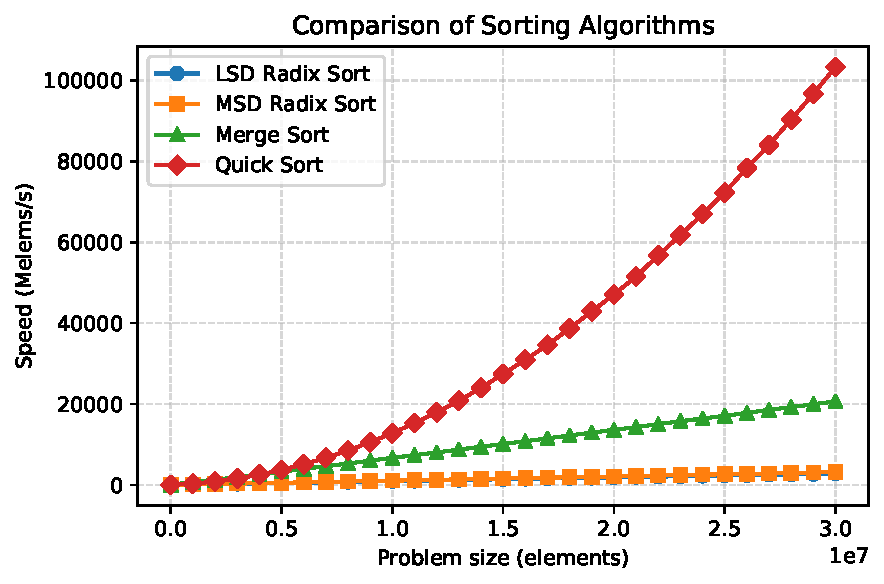
\includegraphics[width=0.8\textwidth]{testingOnSequentialCPU.pdf}
    \caption{Comparison of sorting algorithms}
    \label{fig:testingOnSequentialCPU}
\end{figure}

\subsection{Testing On Parallel CPU}

Here we can see that radix sort on a parallel CPU maintains the linear growth of squeal radix sort. 

\begin{figure}[H]
    \centering
    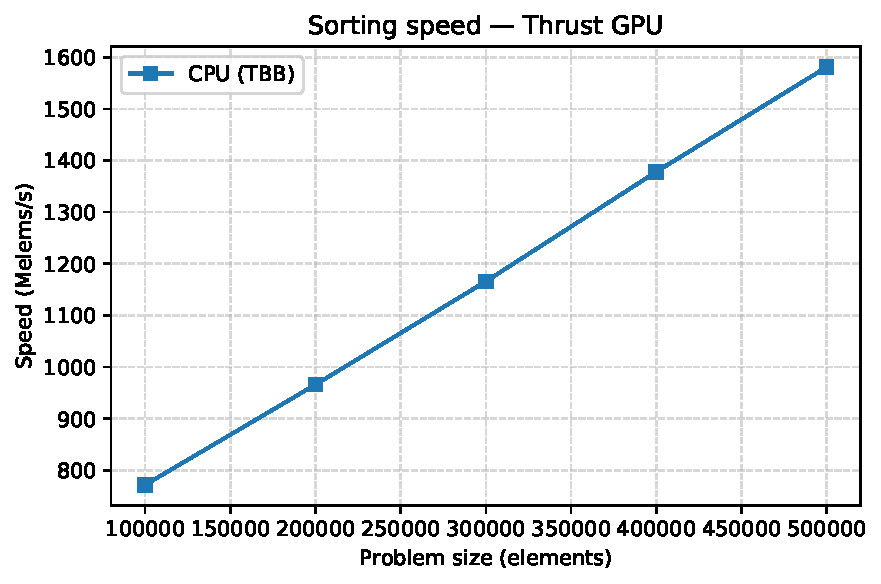
\includegraphics[width=0.8\textwidth]{testingOnParallelCPU.pdf}
    \caption{Sorting speed on CPU with Intel TBB}
    \label{fig:testingOnParallelCPU}
\end{figure}

\subsection{Testing On Parallel GPU}

And on GPUs the growth still stays linear. 

\begin{figure}[H]
    \centering
    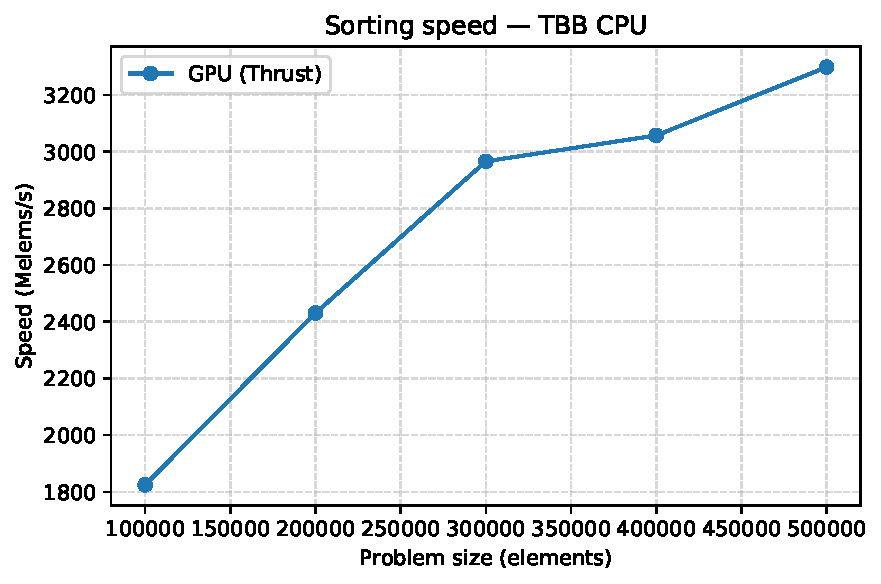
\includegraphics[width=0.8\textwidth]{testingOnParallelGPU.pdf}
    \caption{Sorting speed comparison on GPU with NVIDIA Thrust}
    \label{fig:testignOnParallelGPU}
\end{figure}


\section{Performance On A Heterogeneous System}

An immediate implication from the heterogeneity of processors in a network of computers is that
the processors run at different speeds. A good parallel application for a homogeneous distributed
memory multiprocessor system tries to evenly distribute computations over available processors.

A good parallel application for the heterogeneous platform must distribute computations unevenly,
taking into account the difference in processor speed. The faster the processor is, the more
computations it must perform.

The speed is defined as the number of computation units performed by the processor per one time
unit. The model is application specific. In particular, this means that the computation unit can be
defined differently for different applications --- the important requirement is that the computation
unit does not have to vary during the execution of the application.

\subsection{Data Partitioning}

In High Performance Heterogeneous Computing we are presented with the Functional Performance Model for heterogeneous processors

 \begin{figure}[h]
     \centering
     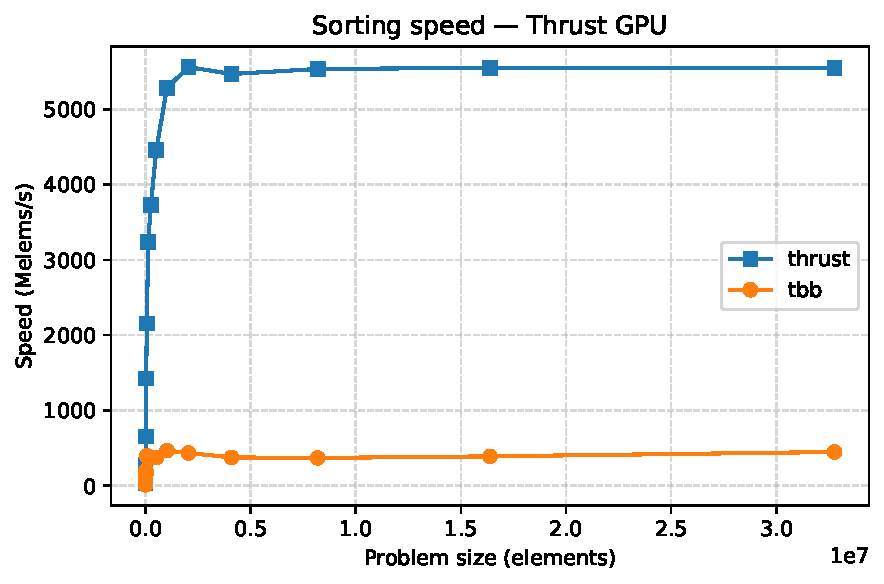
\includegraphics[width=0.8\textwidth]{dataPart.pdf}
     \caption{}
     \label{fig:tbb_results}
 \end{figure}

 However for this specific workload on this specific hardware, the functional model collapses into two simpler two phase strategy: below threshold 1,000,000 use CPU only, above it use a fixed GPU/CPU ratio.

\subsection{Analysis of Heterogeneous Algorithms}

\subsection{Scalability Analysis}

% TODO: Add conclusions

% ─────────────────────────────────────────────
\begin{thebibliography}{9}

\bibitem{nvidia_a40}
NVIDIA Corporation,
\textit{NVIDIA A40 GPU Accelerator Product Brief},
PB-09976-001\_v08, April 2022.

\bibitem{farrelly2024}
S. Farrelly, R. R. Manumachu and A. Lastovetsky,
\textit{OpenH: A Novel Programming Model and API for Developing Portable Parallel Programs
on Heterogeneous Hybrid Servers}, 2024.

\bibitem{chandra2000}
Rohit Chandra,
\textit{Parallel Programming in OpenMP}, 2000.

\bibitem{hoshino}
T. Hoshino, N. Maruyama, S. Matsuoka and R. Takaki,
\textit{CUDA vs OpenACC: Performance Case Studies with Kernel Benchmarks and a
Memory-Bound CFD Application}.

\bibitem{nvidia_nvcc}
NVIDIA Corporation,
\textit{CUDA Compiler Driver NVCC}.

\bibitem{hwu_hajj}
Wen-mei W. Hwu, Izzat El Hajj,
\textit{Programming Massively Parallel Processors}, Chapter 13.

\end{thebibliography}

\end{document}